\documentclass[tikz,border=10pt]{standalone}
\usepackage{tikz}
\usepackage{fontawesome5}
\usepackage{amsmath,amssymb}
\usetikzlibrary{arrows.meta,positioning,fit,backgrounds,calc,shadows,shapes.geometric}

% Color definitions
\definecolor{lavenderDark}{RGB}{15, 44, 89}
\definecolor{lavenderDeep}{RGB}{10, 28, 58}
\definecolor{lavenderMedium}{RGB}{29, 78, 158}
\definecolor{lavenderLight}{RGB}{240, 246, 255}
\definecolor{lavenderBorder}{RGB}{180, 205, 237}
\definecolor{prismNavy}{RGB}{15, 44, 89}
\definecolor{prismBlue}{RGB}{29, 78, 158}
\definecolor{prismTeal}{RGB}{13, 148, 136}
\definecolor{prismGold}{RGB}{217, 119, 6}
\definecolor{prismDark}{RGB}{15, 23, 42}
\definecolor{prismSlate}{RGB}{100, 116, 139}
\definecolor{statusFail}{RGB}{220, 38, 38}
\definecolor{cInput}{RGB}{241, 245, 249}
\definecolor{cStem}{RGB}{224, 242, 254}
\definecolor{cStage1}{RGB}{209, 250, 229}
\definecolor{cStage2}{RGB}{254, 243, 199}
\definecolor{cStage3}{RGB}{254, 226, 226}
\definecolor{cStage4}{RGB}{207, 250, 254}
\definecolor{cHead}{RGB}{219, 234, 254}

\begin{document}
% DenseNet-121 Layer Decomposition and Dense Connectivity Graph
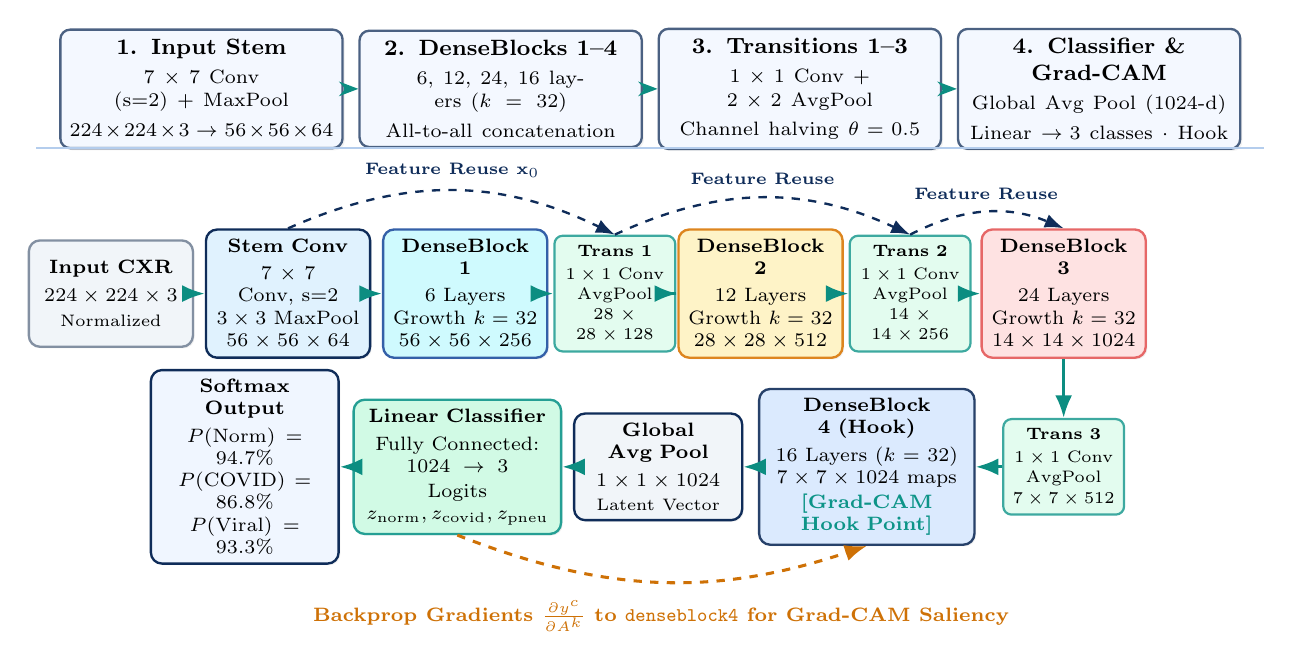
\begin{tikzpicture}[
  x=1cm, y=1cm,
  font=\sffamily,
  dagstep/.style={rectangle, rounded corners=3.5pt, minimum height=1.10cm,
    text width=3.35cm, align=center, draw=lavenderDark!75, fill=lavenderLight!75,
    line width=0.85pt, font=\fontsize{8.2}{9.8}\selectfont\bfseries,
    drop shadow={shadow xshift=0.8pt, shadow yshift=-0.8pt, opacity=0.10}},
  dagarrow/.style={-{Stealth[scale=0.85]}, line width=1.15pt, draw=prismTeal!95!black},
  blkbox/.style={rectangle, rounded corners=4pt, line width=0.85pt,
    minimum height=1.35cm, text width=1.85cm, align=center,
    font=\fontsize{6.8}{8.0}\selectfont, drop shadow={shadow xshift=0.6pt, shadow yshift=-0.6pt, opacity=0.12}},
  transbox/.style={rectangle, rounded corners=3pt, line width=0.80pt,
    draw=prismTeal!80, fill=cStage1!60, minimum height=1.15cm, text width=1.30cm, align=center,
    font=\fontsize{6.2}{7.3}\selectfont},
  skipconn/.style={-{Stealth[scale=0.75]}, line width=0.85pt, draw=prismNavy, dashed}
]

  % Row 1: 4-Stage Architectural Progression
  \node[dagstep] (s1) at (-5.70, 0) {1. Input Stem\\[2pt]\normalfont\fontsize{7.2}{8.5}\selectfont $7\times 7$ Conv (s=2) + MaxPool\\[1pt]$224\times 224\times 3 \to 56\times 56\times 64$};
  \node[dagstep] (s2) at (-1.90, 0) {2. DenseBlocks 1--4\\[2pt]\normalfont\fontsize{7.2}{8.5}\selectfont 6, 12, 24, 16 layers ($k=32$)\\[1pt]All-to-all concatenation};
  \node[dagstep] (s3) at (1.90, 0) {3. Transitions 1--3\\[2pt]\normalfont\fontsize{7.2}{8.5}\selectfont $1\times 1$ Conv + $2\times 2$ AvgPool\\[1pt]Channel halving $\theta=0.5$};
  \node[dagstep] (s4) at (5.70, 0) {4. Classifier \& Grad-CAM\\[2pt]\normalfont\fontsize{7.2}{8.5}\selectfont Global Avg Pool ($1024$-d)\\[1pt]Linear $\to 3$ classes $\cdot$ Hook};

  \draw[dagarrow] (s1) -- (s2);
  \draw[dagarrow] (s2) -- (s3);
  \draw[dagarrow] (s3) -- (s4);

  % Separator
  \draw[draw=lavenderBorder, line width=0.6pt] (-7.8, -0.75) -- (7.8, -0.75);

  % Row 2: Detailed Layer Decomposition Flow (Left-to-Right)
  \node[blkbox, fill=cInput, draw=prismSlate!80] (input_node) at (-6.85, -2.60) {
    \textbf{Input CXR}\\[2pt]
    $224\times 224\times 3$\\[1pt]
    {\fontsize{5.8}{6.8}\selectfont Normalized}
  };

  \node[blkbox, fill=cStem, draw=lavenderDark] (stem_node) at (-4.60, -2.60) {
    \textbf{Stem Conv}\\[2pt]
    $7\times 7$ Conv, s=2\\
    $3\times 3$ MaxPool\\
    $56\times 56\times 64$
  };

  \node[blkbox, fill=cStage4, draw=prismBlue!90] (db1) at (-2.35, -2.60) {
    \textbf{DenseBlock 1}\\[2pt]
    6 Layers\\
    Growth $k=32$\\
    $56\times 56\times 256$
  };

  \node[transbox] (tr1) at (-0.45, -2.60) {
    \textbf{Trans 1}\\[1pt]
    $1\times 1$ Conv\\
    AvgPool\\
    $28\times 28\times 128$
  };

  \node[blkbox, fill=cStage2, draw=prismGold!90] (db2) at (1.40, -2.60) {
    \textbf{DenseBlock 2}\\[2pt]
    12 Layers\\
    Growth $k=32$\\
    $28\times 28\times 512$
  };

  \node[transbox] (tr2) at (3.30, -2.60) {
    \textbf{Trans 2}\\[1pt]
    $1\times 1$ Conv\\
    AvgPool\\
    $14\times 14\times 256$
  };

  \node[blkbox, fill=cStage3, draw=statusFail!70] (db3) at (5.25, -2.60) {
    \textbf{DenseBlock 3}\\[2pt]
    24 Layers\\
    Growth $k=32$\\
    $14\times 14\times 1024$
  };

  % Row 3: Return Flow (Right-to-Left)
  \node[transbox] (tr3) at (5.25, -4.80) {
    \textbf{Trans 3}\\[1pt]
    $1\times 1$ Conv\\
    AvgPool\\
    $7\times 7\times 512$
  };

  \node[blkbox, fill=cHead, draw=lavenderDark!90, text width=2.50cm] (db4) at (2.75, -4.80) {
    \textbf{DenseBlock 4 (Hook)}\\[2pt]
    16 Layers ($k=32$)\\
    $7\times 7\times 1024$ maps\\[1pt]
    {\color{prismTeal}\textbf{[Grad-CAM Hook Point]}}
  };

  \node[blkbox, fill=cInput, draw=prismNavy, text width=1.90cm] (gap) at (0.10, -4.80) {
    \textbf{Global Avg Pool}\\[2pt]
    $1\times 1\times 1024$\\[1pt]
    {\fontsize{5.8}{6.8}\selectfont Latent Vector}
  };

  \node[blkbox, fill=cStage1, draw=prismTeal!90, text width=2.40cm] (head) at (-2.45, -4.80) {
    \textbf{Linear Classifier}\\[2pt]
    Fully Connected: $1024 \to 3$\\[1pt]
    Logits $z_{\text{norm}}, z_{\text{covid}}, z_{\text{pneu}}$
  };

  \node[blkbox, fill=lavenderLight, draw=lavenderDark, text width=2.15cm] (softmax) at (-5.15, -4.80) {
    \textbf{Softmax Output}\\[2pt]
    $P(\text{Norm}) = 94.7\%$\\
    $P(\text{COVID}) = 86.8\%$\\
    $P(\text{Viral}) = 93.3\%$
  };

  % Forward Flow Connections (explicit east to west for row 1, down for turn, east to west for row 2)
  \draw[->, >=Latex, line width=1.15pt, draw=prismTeal!95!black] (input_node.east) -- (stem_node.west);
  \draw[->, >=Latex, line width=1.15pt, draw=prismTeal!95!black] (stem_node.east) -- (db1.west);
  \draw[->, >=Latex, line width=1.15pt, draw=prismTeal!95!black] (db1.east) -- (tr1.west);
  \draw[->, >=Latex, line width=1.15pt, draw=prismTeal!95!black] (tr1.east) -- (db2.west);
  \draw[->, >=Latex, line width=1.15pt, draw=prismTeal!95!black] (db2.east) -- (tr2.west);
  \draw[->, >=Latex, line width=1.15pt, draw=prismTeal!95!black] (tr2.east) -- (db3.west);
  \draw[->, >=Latex, line width=1.15pt, draw=prismTeal!95!black] (db3.south) -- (tr3.north);
  \draw[->, >=Latex, line width=1.15pt, draw=prismTeal!95!black] (tr3.west) -- (db4.east);
  \draw[->, >=Latex, line width=1.15pt, draw=prismTeal!95!black] (db4.west) -- (gap.east);
  \draw[->, >=Latex, line width=1.15pt, draw=prismTeal!95!black] (gap.west) -- (head.east);
  \draw[->, >=Latex, line width=1.15pt, draw=prismTeal!95!black] (head.west) -- (softmax.east);

  % Dense Concatenation Skip Connections (curved lines representing intra-block feature reuse)
  \draw[->, >=Latex, line width=0.85pt, draw=prismNavy, dashed] (stem_node.north) to[bend left=25] node[above=1pt, font=\fontsize{6.0}{7.0}\selectfont\color{prismNavy}\bfseries]{Feature Reuse $\mathbf{x}_0$} (tr1.north);
  \draw[->, >=Latex, line width=0.85pt, draw=prismNavy, dashed] (tr1.north) to[bend left=25] node[above=1pt, font=\fontsize{6.0}{7.0}\selectfont\color{prismNavy}\bfseries]{Feature Reuse} (tr2.north);
  \draw[->, >=Latex, line width=0.85pt, draw=prismNavy, dashed] (tr2.north) to[bend left=25] node[above=1pt, font=\fontsize{6.0}{7.0}\selectfont\color{prismNavy}\bfseries]{Feature Reuse} (db3.north);

  % Backward Hook Arrow from Softmax / Head back to DenseBlock 4
  \draw[->, >=Latex, line width=1.1pt, draw=prismGold!95!black, dashed] 
    (head.south) to[bend right=20] 
    node[below=3pt, font=\fontsize{6.8}{8.0}\selectfont\bfseries\color{prismGold!95!black}]{Backprop Gradients $\frac{\partial y^c}{\partial A^k}$ to \texttt{denseblock4} for Grad-CAM Saliency} 
    (db4.south);

\end{tikzpicture}
\end{document}
